% ### Uses XeLaTeX ### %
% ### Needs beamer-master ### %
\documentclass[aspectratio=169]{beamer} %. Aspect Ratio 16:9
\usetheme{AI2} % beamerthemeSprace.sty
% DATA FOR FOOTER
\date{2019}
\title{}
\author{}
\institute{Advanced Institute for Artificial Intelligence (AI2)}
\begin{document}    
% ####################################
% FIRST SLIDE 						:: \SliTit{<Title of the Talk>}{<Author Name>}{<Intitution>}
% SLIDE SUB-TITLE					:: \SliSubTit{<Title of the Chapter>}{<Title of the Section>}
% SLIDE WITH TITLE 					:: \SliT{<Title>}{Content}
% SLIDE NO TITLE 						:: \Sli{<Content>} 
% SLIDE DOUBLE COLUMN WITH TITLE 	:: \SliDT{<Title>}{<First Column>}{<Second Column>}
% SLIDE DOUBLE COLUMN NO TITLE 		:: \SliD{<First Column>}{<Second Column>}
% SLIDE ADVANCED WITH TITLE 			:: \SliAdvT{<Title>}{<Content>}
% SLIDE ADVANCED  NO TITLE 			:: \SliAdv{<Content>}
% SLIDE ADVANCED DOUBLE TITLE 		:: SliAdvDT{<Title>}{<First Column>}{<Second Column>}
% SLIDE ADVANCED DOUBLE NO TITLE 	:: SliAdvD{<First Column>}{<Second Column>}
% ITEMIZE 							:: \begin{itemize}  \IteOne{1st Level} \IteTwo {2nd Level} \IteThr{3rd Level} \end{itemize}
% SECTION 							:: \secx{Section} | \secxx{Sub-Section}
% COLOR BOX 						:: \blu{blue} + \red{red} + \yel{yellow} + \gre{green}
% FRAME 							:: \fra{sprace} \frab{blue} \frar{red} + \fray{yellow} + \frag{green}	
% REFERENCE						:: \refer{<doi number>}
% FIGURE 							::  \img{X}{Y}{<scale>}{Figures/.png} 
% FIGURE							:: \begin{center}\includegraphics[scale=<#>]{Figures/.png}\end{center}
% PROJECT STATUS					:: \planned\~    \started\~   \underway\~   \done\~   
% EXERCICIO							:: \Exe{<#>}{<text>}
% STACKREL							:: \underset{<down>}{<up>}
% FLUSH LEFT						:: \begin{flalign*}  & <1st equation> & \\  & <12nd equation>  & \\ \end{flalign*}
% REAL / IMAGINAY					:: \Re / \Im
% SLASH								:: \sl{} or \sl
% BOLD MATH							:: \pmb{<>}
% ####################################
%
% FIRST SLIDE :: DO NOT BREAK LINE !!!
\SliTit{SQL}{Advanced Institute for Artificial Intelligence}{https://advancedinstitute.ai}

% SLIDE WITH TITLE
\SliT{Sumário}{

\begin{itemize}
  \IteOne{Introdução}
  \IteOne{Módulos}
  \IteOne{Exemplos}
\end{itemize}

}

% SLIDE WITH TITLE
\SliT{SQL}{
SQL (Structured Query Language)
\begin{itemize}
  \IteOne{Linguagem declarativa para manipulação e recuperação de dados}
  \IteOne{Linguagem padrão para os SGBDs (Sistemas Gerenciadores de Bancos de Dados) relacionais}
\end{itemize}

}

\SliT{SQL}{

Dividida em 4 módulos:

\begin{itemize}
  \IteOne{Linguagem de Defnição de Dados (DDL): Defnir esquemas de relação, excluir relações e modifcar esquemas}
\IteOne{Linguagem de Manipulação de Dados (DML): Inserir, excluir e modifcar dados e linguagem de consulta (Álgebra Relacional)}

\IteOne{Linguagem de Controle de Dados (DCL): Gerenciar aspectos de controle de acesso entre usuários e dados}
\IteOne{Linguagem de Transação de Dados(DTL): Gerenciar aspectos de transações}

\end{itemize}

}

\SliT{SQL}{
DDL
\begin{itemize}
  \IteOne{SGBD possui um ou mais bancos de dados}
  \IteOne{Um banco de dados possui uma ou mais tabelas}
  \IteOne{Uma tabela possui:}
  \IteTwo{Uma ou mais colunas}
  \IteTwo{Possui um índice primário. Um índice é um valor que identifica uma linha da tabela unicamente, portanto não pode ser repetido}
  
\end{itemize}

}

\SliT{Ciência dos Dados}{
\begin{center}
    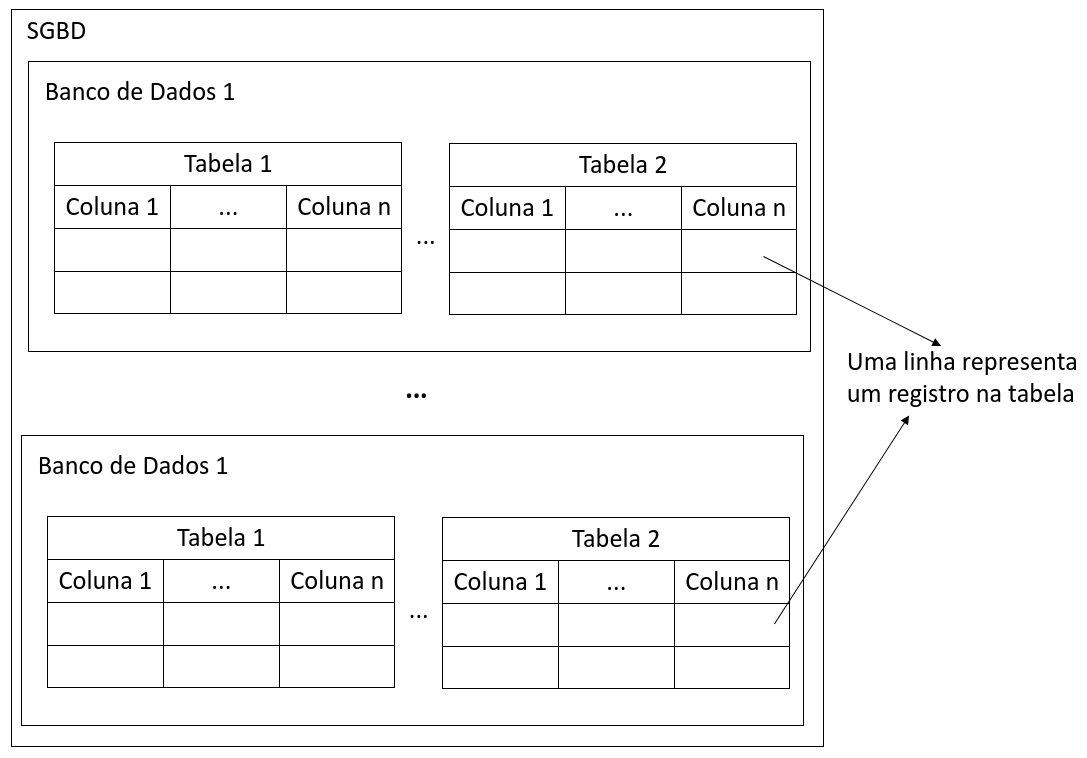
\includegraphics[scale=0.27]{vv.png}     
    \end{center}
}

\SliT{SQL}{
DDL
\begin{itemize}
  \IteOne{CREATE: Cria um objeto dentro da base de dados}
  \IteOne{ALTER: Altera um objeto já existente}
  \IteOne{DROP: Apaga um objeto do banco de dados}
\end{itemize}

}

\SliT{SQL}{
DDL
\begin{itemize}
  \IteOne{CREATE DATABASE (nome do banco) }
  \IteOne{CREATE TABLE (tabela) ((campo1) (tipo),[..., (campo n) (tipo)]PRIMARY KEY (coluna)FOREIGN KEY (coluna) REFERENCES (tabela ref)((coluna ref)))}
  \IteTwo{PRIMARY KEY: Restrição de chave primária}
  \IteTwo{FOREIGN KEY: Restrição de chave estrangeira}
\end{itemize}

}

\SliT{SQL}{
DDL
\begin{itemize}
  \IteOne{ALTER TABLE (tabela) ADD (coluna)(tipo) }
  \IteOne{ALTER TABLE (tabela) DROP (coluna)}
  \IteOne{DROP TABLE (tabela)}
\end{itemize}
}


\SliT{SQL}{
DML
\begin{itemize}
  \IteOne{INSERT : inserir registros }
  \IteOne{UPDATE : atualiza registros}
  \IteOne{DELETE : remover registros}
  \IteOne{SELECT : consultar registros}
\end{itemize}
}

\SliT{SQL}{
DML
\begin{itemize}
  \IteOne{INSERT INTO tabela (campo1, campo2, ..., campon) VALUES (valor1, valor2, ..., valorn)}
  \IteOne{UPDATE tabela SET campo1 = valor1 [, ..., campo n valor n ]WHERE condição}
  \IteOne{DELETE FROM tabela WHERE condição}
  \IteOne{SELECT [ lista de atributos] FROM lista de tabelas] WHERE condição}
\end{itemize}
}

\SliT{SQL}{
Inserção de Dados
\begin{itemize}
  \IteOne{Inserção de dados pode ser feita via comando SQL ou por scripts contendo diversas inserções}
  \IteOne{O Conteúdo de um banco pode ser recuperado para um CSV}
  \IteOne{Arquivos CSV também podem ser usados para atualizar registros em um Banco de Dados}

\end{itemize}
}

\SliT{SQL}{
Operações com Seleção de Dados
\begin{itemize}
  \IteOne{Filtro por colunas}
  \IteOne{Filtro por registros}
  \IteOne{Classificação de registros}
  \IteOne{Agrupamento de registros em uma tabela}
  \IteOne{Unificação de tabelas}
\end{itemize}
}

\end{document}